\documentclass[10pt]{article}
\usepackage[margin=20mm]{geometry}
\usepackage{amsmath,amssymb,booktabs,tikz,graphicx,hyperref,xurl}
\hypersetup{colorlinks=true,urlcolor=blue}
\title{Actual local-series bridge for the common rational denominator}
\author{Producer proof report; unsigned PCC standing}
\date{8 November 2026}
\begin{document}\maketitle
The actual common denominator now has an integral formal-series inverse,
connected to the imported kernel definition at every scale and source node.
The earlier generic polynomial-degree bound is also connected to the actual
kernel. These are symbolic proofs; no new experiment or benchmark was run.
All results here carry \texttt{[pcc:unverified]} standing pending a trusted
signature. The original frozen panel, its losses and its PDF remain intact.

\section*{Concrete local ring and actual product identity}
Set $N=2^{a+1}$, $L=2^a$, and $m,s\in\operatorname{Fin}N$.
The coefficient ring is the concrete subring
\[A=\{r\in\mathbb Q:\lvert r\rvert_2\le1\}.\]
For $j\ne m$, $0<|m-j|<N$ implies $v_2(m-j)<a+1$:
the integer $2^{v_2(m-j)}$ divides $|m-j|$. Thus
$c_{m,j}=N/(m-j)\in A$. The actual source normalizer $\rho_m$ and its
reciprocal lie in $A$; \texttt{rhoUnit} packages them as a unit.
\texttt{LocalIntegral.grid\_ratio\_integral} proves the grid statement.

From the actual punctured-product definition, for \emph{every rational} $z$,
\[ B_s(m-L+Nz)=\rho_m
 \begin{cases}1&s=m,\\c_{m,s}z&s\ne m\end{cases}
 \prod_{j\ne m,s}(1+c_{m,j}z).\]
\texttt{LocalCharts.actual\_chart\_formula} proves this identity;
\texttt{localBase\_eval} identifies the explicit $A$-polynomial with the
imported \texttt{baseKernel}. No unit-normalizer or polynomial-representation
hypothesis is delegated to the caller. The earlier module only adds an
exposed exact product API; its mathematical definition is unchanged.

\section*{Actual denominator and integral inverse}
Let $P_m=\sum_s\mathrm{localBase}_{m,s}$. Then
\[P_m(z)=D(m-L+Nz),\qquad D(T)=\sum_s B_s(T),\qquad P_m(0)=\rho_m.\]
The first equality holds for all rational $z$. The constant coefficient is a
unit, so formal inversion over $A$ constructs $Q_m\in A[[X]]$ with
\[P_m Q_m=Q_mP_m=1.\]
The theorem \texttt{actual\_integral\_denominator\_inverse} states existence
of the actual representative and inverse. It assumes neither integrality of
an unspecified series nor a denominator-unit hypothesis.

Define $U_{m,s}=\mathrm{localBase}_{m,s}^{\,2}Q_m$.
\texttt{localKernel\_identity} proves $P_mU_{m,s}=\mathrm{localBase}_{m,s}^{\,2}$.
All reciprocal and kernel coefficients belong to $A$, hence their rational
two-adic norms are at most one. This is a coefficientwise formal-series
statement; it does not assert analytic convergence at arbitrary rational $z$.
Claims \texttt{PCC-20261108-1270b2} and \texttt{PCC-20261108-ad84dd} pin these
statements and their exact hypotheses.

\newpage
\section*{Source-connected proof chain}
\begin{center}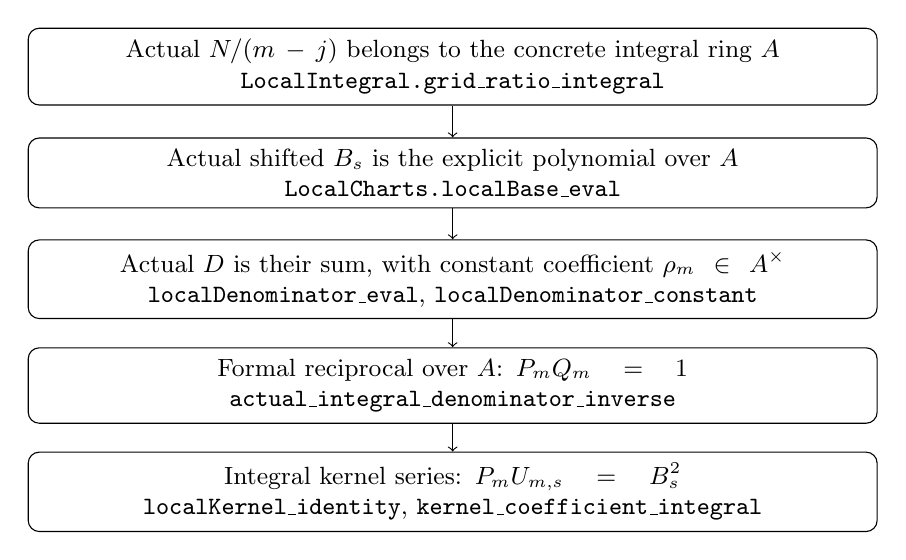
\begin{tikzpicture}[every node/.style={draw,rounded corners,align=center,text width=10.5cm,font=\small,inner sep=4pt},node distance=1.35cm]
\node (a) {Actual $N/(m-j)$ belongs to the concrete integral ring $A$\\\texttt{LocalIntegral.grid\_ratio\_integral}};
\node[below of=a] (b) {Actual shifted $B_s$ is the explicit polynomial over $A$\\\texttt{LocalCharts.localBase\_eval}};
\node[below of=b] (c) {Actual $D$ is their sum, with constant coefficient $\rho_m\in A^\times$\\\texttt{localDenominator\_eval}, \texttt{localDenominator\_constant}};
\node[below of=c] (d) {Formal reciprocal over $A$: $P_m Q_m=1$\\\texttt{actual\_integral\_denominator\_inverse}};
\node[below of=d] (e) {Integral kernel series: $P_m U_{m,s}=B_s^2$\\\texttt{localKernel\_identity}, \texttt{kernel\_coefficient\_integral}};
\draw[->] (a)--(b);\draw[->](b)--(c);\draw[->](c)--(d);\draw[->](d)--(e);
\end{tikzpicture}\end{center}
The arrows are proved links to actual objects, not measured correlations.
The proof map and source are in \path{lean/LOCAL_SERIES_PROOF_MAP.md}.

\section*{Actual global degree and local precision}
\texttt{GlobalPolynomials.basePolynomial} is the actual puncture polynomial
with its actual center denominator. Its evaluation equals imported
\texttt{baseKernel} for every rational $T$. Its degree is at most $N-1$,
and a finite product of its squares has degree at most $2|E|(N-1)$.
This closes the earlier generic-degree bridge; it does not prove fixed-edge
homogeneity of the actual recursive contraction program.
Claim \texttt{PCC-20261108-ee5503} records this scope.

The instantiated inverse coefficient recurrence uses only earlier inverse
coefficients. If an ideal $I$ satisfies $E-P_m\in I$ and an approximation has
an exact inverse $EF=1$, then
\[F-Q_m=F(P_m-E)Q_m\in I.\]
\texttt{LocalPrecision.inverse\_jet\_stability} takes
$I=(2^p,X^q)\subset A[[X]]$. There is no extra precision loss in this
algebraic congruence. Both input congruence and $EF=1$ remain explicit
hypotheses. Equivalence to a concrete finite buffer, its executable inverse,
and full Hermite recovery are still separate. Claim
\texttt{PCC-20261108-78ae71} pins the conditional theorem.

\section*{Checks, provenance and continuation}
The pinned Lean project builds these modules; actual source-gate and official
import-inclusive fresh-check receipts are recorded in
\path{lean/LOCAL_SERIES_VERIFICATION.md}. Only standard Lean foundations are
allowed. All failed builds are retained. KB tools were unavailable (status127);
the reviewed primary sources are the pinned Mathlib norm, valuation,
polynomial and power-series APIs plus the actual prior kernel and recovery
sources. No priority or literature-exhaustion claim is made.

The original eight unsigned ledger events were preserved verbatim and in Git
while merging concurrent main registrations. Main remains the byte prefix;
unchanged local event bodies were appended by the maintained routine, with
old/new hashes in \path{pcc-reconciliation/reapplied-events.json}.

Next: concrete finite-buffer congruence, actual contraction homogeneity,
finite-precision recovery and fully charged construction/child-entry costs
with a uniform all-level mode bound. Formal series existence alone supplies
neither that evaluator nor its cost recurrence. See \path{PLAN.md}.
\end{document}
